% Options for packages loaded elsewhere
\PassOptionsToPackage{unicode}{hyperref}
\PassOptionsToPackage{hyphens}{url}
\PassOptionsToPackage{dvipsnames,svgnames,x11names}{xcolor}
%
\documentclass[
  letterpaper,
  DIV=11,
  numbers=noendperiod]{scrartcl}

\usepackage{amsmath,amssymb}
\usepackage{iftex}
\ifPDFTeX
  \usepackage[T1]{fontenc}
  \usepackage[utf8]{inputenc}
  \usepackage{textcomp} % provide euro and other symbols
\else % if luatex or xetex
  \usepackage{unicode-math}
  \defaultfontfeatures{Scale=MatchLowercase}
  \defaultfontfeatures[\rmfamily]{Ligatures=TeX,Scale=1}
\fi
\usepackage{lmodern}
\ifPDFTeX\else  
    % xetex/luatex font selection
\fi
% Use upquote if available, for straight quotes in verbatim environments
\IfFileExists{upquote.sty}{\usepackage{upquote}}{}
\IfFileExists{microtype.sty}{% use microtype if available
  \usepackage[]{microtype}
  \UseMicrotypeSet[protrusion]{basicmath} % disable protrusion for tt fonts
}{}
\makeatletter
\@ifundefined{KOMAClassName}{% if non-KOMA class
  \IfFileExists{parskip.sty}{%
    \usepackage{parskip}
  }{% else
    \setlength{\parindent}{0pt}
    \setlength{\parskip}{6pt plus 2pt minus 1pt}}
}{% if KOMA class
  \KOMAoptions{parskip=half}}
\makeatother
\usepackage{xcolor}
\setlength{\emergencystretch}{3em} % prevent overfull lines
\setcounter{secnumdepth}{-\maxdimen} % remove section numbering
% Make \paragraph and \subparagraph free-standing
\makeatletter
\ifx\paragraph\undefined\else
  \let\oldparagraph\paragraph
  \renewcommand{\paragraph}{
    \@ifstar
      \xxxParagraphStar
      \xxxParagraphNoStar
  }
  \newcommand{\xxxParagraphStar}[1]{\oldparagraph*{#1}\mbox{}}
  \newcommand{\xxxParagraphNoStar}[1]{\oldparagraph{#1}\mbox{}}
\fi
\ifx\subparagraph\undefined\else
  \let\oldsubparagraph\subparagraph
  \renewcommand{\subparagraph}{
    \@ifstar
      \xxxSubParagraphStar
      \xxxSubParagraphNoStar
  }
  \newcommand{\xxxSubParagraphStar}[1]{\oldsubparagraph*{#1}\mbox{}}
  \newcommand{\xxxSubParagraphNoStar}[1]{\oldsubparagraph{#1}\mbox{}}
\fi
\makeatother

\usepackage{color}
\usepackage{fancyvrb}
\newcommand{\VerbBar}{|}
\newcommand{\VERB}{\Verb[commandchars=\\\{\}]}
\DefineVerbatimEnvironment{Highlighting}{Verbatim}{commandchars=\\\{\}}
% Add ',fontsize=\small' for more characters per line
\usepackage{framed}
\definecolor{shadecolor}{RGB}{241,243,245}
\newenvironment{Shaded}{\begin{snugshade}}{\end{snugshade}}
\newcommand{\AlertTok}[1]{\textcolor[rgb]{0.68,0.00,0.00}{#1}}
\newcommand{\AnnotationTok}[1]{\textcolor[rgb]{0.37,0.37,0.37}{#1}}
\newcommand{\AttributeTok}[1]{\textcolor[rgb]{0.40,0.45,0.13}{#1}}
\newcommand{\BaseNTok}[1]{\textcolor[rgb]{0.68,0.00,0.00}{#1}}
\newcommand{\BuiltInTok}[1]{\textcolor[rgb]{0.00,0.23,0.31}{#1}}
\newcommand{\CharTok}[1]{\textcolor[rgb]{0.13,0.47,0.30}{#1}}
\newcommand{\CommentTok}[1]{\textcolor[rgb]{0.37,0.37,0.37}{#1}}
\newcommand{\CommentVarTok}[1]{\textcolor[rgb]{0.37,0.37,0.37}{\textit{#1}}}
\newcommand{\ConstantTok}[1]{\textcolor[rgb]{0.56,0.35,0.01}{#1}}
\newcommand{\ControlFlowTok}[1]{\textcolor[rgb]{0.00,0.23,0.31}{\textbf{#1}}}
\newcommand{\DataTypeTok}[1]{\textcolor[rgb]{0.68,0.00,0.00}{#1}}
\newcommand{\DecValTok}[1]{\textcolor[rgb]{0.68,0.00,0.00}{#1}}
\newcommand{\DocumentationTok}[1]{\textcolor[rgb]{0.37,0.37,0.37}{\textit{#1}}}
\newcommand{\ErrorTok}[1]{\textcolor[rgb]{0.68,0.00,0.00}{#1}}
\newcommand{\ExtensionTok}[1]{\textcolor[rgb]{0.00,0.23,0.31}{#1}}
\newcommand{\FloatTok}[1]{\textcolor[rgb]{0.68,0.00,0.00}{#1}}
\newcommand{\FunctionTok}[1]{\textcolor[rgb]{0.28,0.35,0.67}{#1}}
\newcommand{\ImportTok}[1]{\textcolor[rgb]{0.00,0.46,0.62}{#1}}
\newcommand{\InformationTok}[1]{\textcolor[rgb]{0.37,0.37,0.37}{#1}}
\newcommand{\KeywordTok}[1]{\textcolor[rgb]{0.00,0.23,0.31}{\textbf{#1}}}
\newcommand{\NormalTok}[1]{\textcolor[rgb]{0.00,0.23,0.31}{#1}}
\newcommand{\OperatorTok}[1]{\textcolor[rgb]{0.37,0.37,0.37}{#1}}
\newcommand{\OtherTok}[1]{\textcolor[rgb]{0.00,0.23,0.31}{#1}}
\newcommand{\PreprocessorTok}[1]{\textcolor[rgb]{0.68,0.00,0.00}{#1}}
\newcommand{\RegionMarkerTok}[1]{\textcolor[rgb]{0.00,0.23,0.31}{#1}}
\newcommand{\SpecialCharTok}[1]{\textcolor[rgb]{0.37,0.37,0.37}{#1}}
\newcommand{\SpecialStringTok}[1]{\textcolor[rgb]{0.13,0.47,0.30}{#1}}
\newcommand{\StringTok}[1]{\textcolor[rgb]{0.13,0.47,0.30}{#1}}
\newcommand{\VariableTok}[1]{\textcolor[rgb]{0.07,0.07,0.07}{#1}}
\newcommand{\VerbatimStringTok}[1]{\textcolor[rgb]{0.13,0.47,0.30}{#1}}
\newcommand{\WarningTok}[1]{\textcolor[rgb]{0.37,0.37,0.37}{\textit{#1}}}

\providecommand{\tightlist}{%
  \setlength{\itemsep}{0pt}\setlength{\parskip}{0pt}}\usepackage{longtable,booktabs,array}
\usepackage{calc} % for calculating minipage widths
% Correct order of tables after \paragraph or \subparagraph
\usepackage{etoolbox}
\makeatletter
\patchcmd\longtable{\par}{\if@noskipsec\mbox{}\fi\par}{}{}
\makeatother
% Allow footnotes in longtable head/foot
\IfFileExists{footnotehyper.sty}{\usepackage{footnotehyper}}{\usepackage{footnote}}
\makesavenoteenv{longtable}
\usepackage{graphicx}
\makeatletter
\def\maxwidth{\ifdim\Gin@nat@width>\linewidth\linewidth\else\Gin@nat@width\fi}
\def\maxheight{\ifdim\Gin@nat@height>\textheight\textheight\else\Gin@nat@height\fi}
\makeatother
% Scale images if necessary, so that they will not overflow the page
% margins by default, and it is still possible to overwrite the defaults
% using explicit options in \includegraphics[width, height, ...]{}
\setkeys{Gin}{width=\maxwidth,height=\maxheight,keepaspectratio}
% Set default figure placement to htbp
\makeatletter
\def\fps@figure{htbp}
\makeatother

\usepackage{fontspec}
\usepackage{multirow}
\usepackage{multicol}
\usepackage{colortbl}
\usepackage{hhline}
\newlength\Oldarrayrulewidth
\newlength\Oldtabcolsep
\usepackage{longtable}
\usepackage{array}
\usepackage{hyperref}
\usepackage{float}
\usepackage{wrapfig}
\KOMAoption{captions}{tableheading}
\makeatletter
\@ifpackageloaded{tcolorbox}{}{\usepackage[skins,breakable]{tcolorbox}}
\@ifpackageloaded{fontawesome5}{}{\usepackage{fontawesome5}}
\definecolor{quarto-callout-color}{HTML}{909090}
\definecolor{quarto-callout-note-color}{HTML}{0758E5}
\definecolor{quarto-callout-important-color}{HTML}{CC1914}
\definecolor{quarto-callout-warning-color}{HTML}{EB9113}
\definecolor{quarto-callout-tip-color}{HTML}{00A047}
\definecolor{quarto-callout-caution-color}{HTML}{FC5300}
\definecolor{quarto-callout-color-frame}{HTML}{acacac}
\definecolor{quarto-callout-note-color-frame}{HTML}{4582ec}
\definecolor{quarto-callout-important-color-frame}{HTML}{d9534f}
\definecolor{quarto-callout-warning-color-frame}{HTML}{f0ad4e}
\definecolor{quarto-callout-tip-color-frame}{HTML}{02b875}
\definecolor{quarto-callout-caution-color-frame}{HTML}{fd7e14}
\makeatother
\makeatletter
\@ifpackageloaded{caption}{}{\usepackage{caption}}
\AtBeginDocument{%
\ifdefined\contentsname
  \renewcommand*\contentsname{Tabla de contenidos}
\else
  \newcommand\contentsname{Tabla de contenidos}
\fi
\ifdefined\listfigurename
  \renewcommand*\listfigurename{Listado de Figuras}
\else
  \newcommand\listfigurename{Listado de Figuras}
\fi
\ifdefined\listtablename
  \renewcommand*\listtablename{Lista de Cuadros}
\else
  \newcommand\listtablename{Lista de Cuadros}
\fi
\ifdefined\figurename
  \renewcommand*\figurename{Figura}
\else
  \newcommand\figurename{Figura}
\fi
\ifdefined\tablename
  \renewcommand*\tablename{Cuadro}
\else
  \newcommand\tablename{Cuadro}
\fi
}
\@ifpackageloaded{float}{}{\usepackage{float}}
\floatstyle{ruled}
\@ifundefined{c@chapter}{\newfloat{codelisting}{h}{lop}}{\newfloat{codelisting}{h}{lop}[chapter]}
\floatname{codelisting}{Listado}
\newcommand*\listoflistings{\listof{codelisting}{Listado de Listados}}
\makeatother
\makeatletter
\makeatother
\makeatletter
\@ifpackageloaded{caption}{}{\usepackage{caption}}
\@ifpackageloaded{subcaption}{}{\usepackage{subcaption}}
\makeatother
\ifLuaTeX
\usepackage[bidi=basic]{babel}
\else
\usepackage[bidi=default]{babel}
\fi
\babelprovide[main,import]{spanish}
% get rid of language-specific shorthands (see #6817):
\let\LanguageShortHands\languageshorthands
\def\languageshorthands#1{}
\ifLuaTeX
  \usepackage{selnolig}  % disable illegal ligatures
\fi
\usepackage{bookmark}

\IfFileExists{xurl.sty}{\usepackage{xurl}}{} % add URL line breaks if available
\urlstyle{same} % disable monospaced font for URLs
\hypersetup{
  pdftitle={Masa para Pizza},
  pdfauthor={Miguel Equihua},
  pdflang={es},
  colorlinks=true,
  linkcolor={blue},
  filecolor={Maroon},
  citecolor={Blue},
  urlcolor={Blue},
  pdfcreator={LaTeX via pandoc}}

\title{Masa para Pizza}
\author{Miguel Equihua}
\date{Xalapa, Ver., 20 de junio, 2024}

\begin{document}
\maketitle

\renewcommand*\contentsname{Tabla de contenidos}
{
\hypersetup{linkcolor=}
\setcounter{tocdepth}{3}
\tableofcontents
}
\listoftables
En esta libreta \emph{RMarkdown} les comparto mis notas de lo que hice
en relación con los datos de masa para pizza.

El Estudio de Marcelo es un experimento \emph{completamente
aleatorizado}, no hubo restricciones a la aleatorización como para
producir \textbf{bloques} o división en parcelas (\textbf{parcela
dividida}). Los tratamientos los ideó Marcelo como tratamientos
factoriales, resultado de la combinación de cantidades variables de
azúcar y leche, pero finalmente optó por tratarlas como una serie de
recetas (sin decirnos que cantidad de leche o azúcar empleo, típico de
los cocineros, guardar secretos), así que no nos queda otra que tratar
al arreglo de tratamientos como una clasificación simple en
\emph{recetas} (ANOVA de una sola vía dirían otros). El modelo que
describe esto es algo así (Ecuación~\ref{eq-mod-est-lin}):

\begin{equation}\phantomsection\label{eq-mod-est-lin}{
y_{ij} = \mu + R_i + \varepsilon_{j(i)}
}\end{equation}

En donde \emph{i} tiene 4 niveles, uno por cada receta, \emph{j} tiene 4
niveles, por el número de repeticiones de cada receta. Por lo tanto, los
grados de libertad en el cuadro de análisis de la varianza deben ser 3
para las recetas y 12 para el error.

\subsection{Exploración tabular de los
datos}\label{exploraciuxf3n-tabular-de-los-datos}

Una vez leídos los datos del archivo plano \emph{texto separado por
comas}, con acrónimo csv), definí la columna \emph{recetas} como
\emph{factor}, lo hice con la función \texttt{mutate} para interactuar
con la tabla completa. Me asomé a los datos calculando los promedios por
tratamiento. Seguí la metáfora de \emph{tubos} con ayuda de la
biblioteca \texttt{tidyverse} o \texttt{dplyr}.

\begin{Shaded}
\begin{Highlighting}[]
\CommentTok{\#pizzas \textless{}{-} list.files(".", pattern = "\^{}masa{-}para", recursive = T, full.names = T)}
\CommentTok{\#masa\_2 \textless{}{-} read\_csv(pizzas, col\_names = TRUE)}

\NormalTok{url\_datos }\OtherTok{\textless{}{-}} \StringTok{"https://drive.google.com/file/d/1uVUOqwobv67E5xTsSSxjg9f9qypW{-}aIS/view"}
\NormalTok{dat\_datos\_id }\OtherTok{\textless{}{-}} \FunctionTok{str\_extract}\NormalTok{(url\_datos, }\StringTok{"(?\textless{}=d/)(.*)(?=/view)"}\NormalTok{)}

\NormalTok{url\_drive }\OtherTok{\textless{}{-}} \StringTok{"https://docs.google.com/uc?id=\%s\&export=download"} 
\NormalTok{masa }\OtherTok{\textless{}{-}} \FunctionTok{read.csv}\NormalTok{(}\FunctionTok{sprintf}\NormalTok{(url\_drive, dat\_datos\_id)) }

\NormalTok{masa }\SpecialCharTok{\%\textgreater{}\%}
  \FunctionTok{mutate}\NormalTok{(}\AttributeTok{receta =} \FunctionTok{factor}\NormalTok{(receta)) }\SpecialCharTok{\%\textgreater{}\%}            
  \FunctionTok{arrange}\NormalTok{(receta) }\OtherTok{{-}\textgreater{}}\NormalTok{ masa }\CommentTok{\# también puedo guardar resultados así}

\NormalTok{masa }\SpecialCharTok{\%\textgreater{}\%} 
  \FunctionTok{group\_by}\NormalTok{(receta) }\SpecialCharTok{\%\textgreater{}\%} 
  \FunctionTok{summarise}\NormalTok{(}\AttributeTok{media =} \FunctionTok{mean}\NormalTok{(tiempo, }\AttributeTok{na.rm =} \ConstantTok{TRUE}\NormalTok{), }
            \AttributeTok{mediana =} \FunctionTok{median}\NormalTok{(tiempo, }\AttributeTok{na.rm =} \ConstantTok{TRUE}\NormalTok{),}
            \AttributeTok{var =} \FunctionTok{var}\NormalTok{(tiempo)) }
\end{Highlighting}
\end{Shaded}

\begin{verbatim}
# A tibble: 4 x 4
  receta media mediana   var
  <fct>  <dbl>   <dbl> <dbl>
1 " A"    486.    488. 6340.
2 " B"    196.    192. 4490.
3 " C"    656     675  5491.
4 " D"    184.    175  2723.
\end{verbatim}

Recetas es ahora un factor, esto implica que es un tipo especial de
variable que al incorporarla en un modelo estadístico se suele
desagregar en una colección de variables indicadoras o \textbf{dummy}
que tienen el papel \emph{en conjunto} de modelar el efecto de
condiciones que se reconocen en forma cualitativa. Así, lo que hace el
modelo es responder a la indicación de \textbf{presencia} del
tratamiento indicado. L estructura que en \emph{R} se define como
\texttt{factor} es entonces un forma compacta de recoger esa indicación
de cuándo está presente cada tratamiento en la estructura de datos. Una
idea general de cómo funcional las variables indicadoras se ilustra en
el Cuadro~\ref{tbl-dummy}
(\href{https://quarto.org/docs/authoring/tables.html}{opciones de
formateo de tablas aquí}).

\begin{table}

\caption{\label{tbl-dummy}Variables indicadoras derivadas del factor
\emph{receta}.}

\begin{minipage}{0.33\linewidth}
~\end{minipage}%
%
\begin{minipage}{0.33\linewidth}

\begin{longtable}[]{@{}llll@{}}
\toprule\noalign{}
A & B & C & D \\
\midrule\noalign{}
\endhead
\bottomrule\noalign{}
\endlastfoot
1 & 0 & 0 & 0 \\
0 & 1 & 0 & 0 \\
0 & 0 & 1 & 0 \\
0 & 0 & 0 & 1 \\
\end{longtable}

\end{minipage}%
%
\begin{minipage}{0.33\linewidth}
~\end{minipage}%

\end{table}%

\subsection{Exploración gráfica}\label{exploraciuxf3n-gruxe1fica}

Use una gráfica simple con letras para las recetas para tener una idea
de los datos. Usé la función \texttt{unclass}para obtener un índice
numérico asociado con las recetas, así le doy fácilmente un color
distinto a cada receta, aunque son los colores que sean, podría hacer
algo semejante para escoger los colores de mi gusto o incluso hacer un
vector de colores por nombre, pero para el caso exploratorio esto que
hice es muy fácil y rápido.

\begin{Shaded}
\begin{Highlighting}[]
\FunctionTok{plot}\NormalTok{(masa}\SpecialCharTok{$}\NormalTok{tiempo, }\AttributeTok{type =} \StringTok{"n"}\NormalTok{, }\AttributeTok{ylab =} \StringTok{"tiempo"}\NormalTok{)}
\FunctionTok{text}\NormalTok{(masa}\SpecialCharTok{$}\NormalTok{tiempo, }\AttributeTok{labels =}\NormalTok{ masa}\SpecialCharTok{$}\NormalTok{receta,}
     \AttributeTok{col =} \FunctionTok{as.integer}\NormalTok{(}\FunctionTok{unclass}\NormalTok{(masa}\SpecialCharTok{$}\NormalTok{receta)))}
\end{Highlighting}
\end{Shaded}

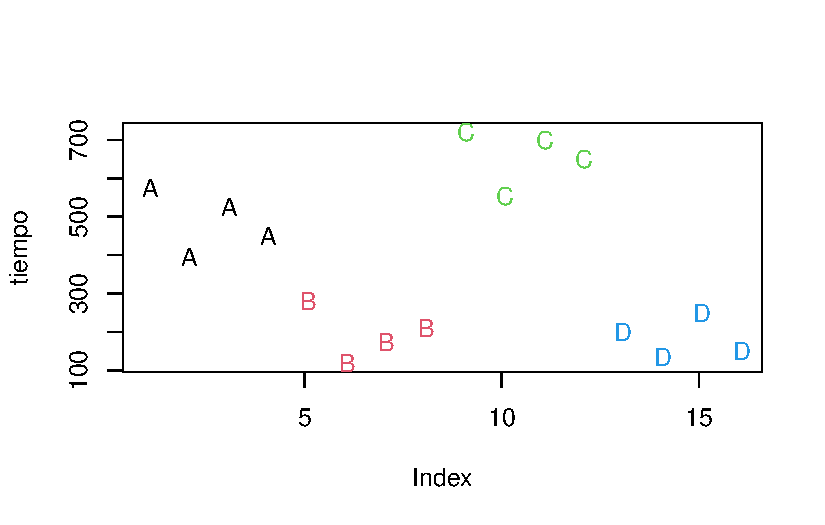
\includegraphics{solucion-masa-pizza_files/figure-pdf/explora-1.pdf}

Si quisiéramos hacer una gráfica más profesional podemos usar
\texttt{ggplot2} en la forma siguiente: 1) datos, los de masa, 2)
arreglo (\emph{estética}) x=recetas, y=tiempo y colorear según recetas,
finalmente 3) la geometría de la gráfica: representa los datos como
puntos.

\begin{Shaded}
\begin{Highlighting}[]
\FunctionTok{ggplot}\NormalTok{(masa, }\FunctionTok{aes}\NormalTok{(}\AttributeTok{x =}\NormalTok{ receta, }\AttributeTok{y =}\NormalTok{ tiempo, }\AttributeTok{colour =}\NormalTok{ receta)) }\SpecialCharTok{+}
  \FunctionTok{geom\_point}\NormalTok{(}\AttributeTok{size =} \DecValTok{3}\NormalTok{, }\AttributeTok{show.legend =} \ConstantTok{FALSE}\NormalTok{)}
\end{Highlighting}
\end{Shaded}

\begin{figure}[H]

\centering{

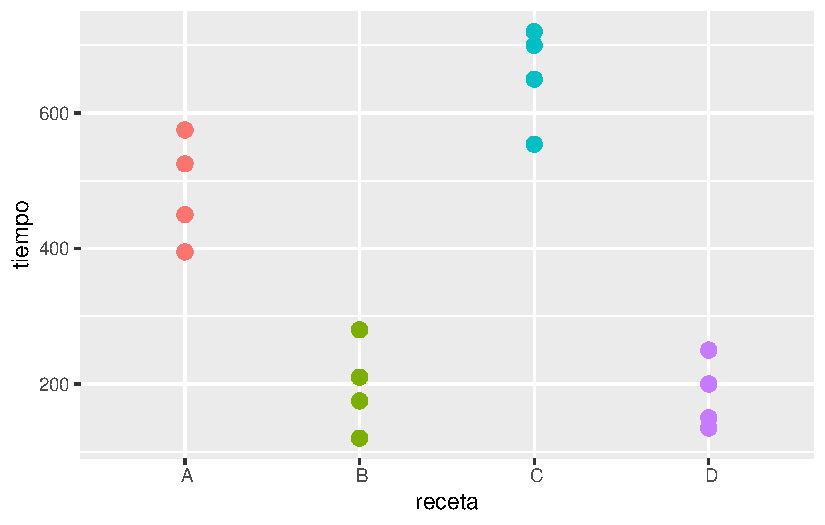
\includegraphics{solucion-masa-pizza_files/figure-pdf/fig-ggp-explora-1.pdf}

}

\caption{\label{fig-ggp-explora}Velocidad de leudado de masa de pizza}

\end{figure}%

\subsection{Prueba de hipótesis}\label{prueba-de-hipuxf3tesis}

Me parece que hay buenas razones para pensar que puede detectarse un
efecto importante de alguna de las recetas. No encuentro a simple vista
mayores razones para pensar que haya heterogeneidad de varianzas o falta
de normalidad, aunque los tratamientos de menor tiempo se ven algo más
compactos que los más lentos (típico patrón que conduce a la
\emph{heterocedasticidad}, asociación de la varianza y la media). Pero
empezaré con lo más simple.

\begin{Shaded}
\begin{Highlighting}[]
\NormalTok{masa\_lm }\OtherTok{\textless{}{-}} \FunctionTok{lm}\NormalTok{(tiempo }\SpecialCharTok{\textasciitilde{}}\NormalTok{ receta, }\AttributeTok{data =}\NormalTok{ masa)}
\FunctionTok{anova}\NormalTok{(masa\_lm)}
\end{Highlighting}
\end{Shaded}

\begin{verbatim}
Analysis of Variance Table

Response: tiempo
          Df Sum Sq Mean Sq F value   Pr(>F)    
receta     3 638968  212989  44.739 8.64e-07 ***
Residuals 12  57128    4761                     
---
Signif. codes:  0 '***' 0.001 '**' 0.01 '*' 0.05 '.' 0.1 ' ' 1
\end{verbatim}

\begin{Shaded}
\begin{Highlighting}[]
\FunctionTok{summary}\NormalTok{(masa\_lm)}
\end{Highlighting}
\end{Shaded}

\begin{verbatim}

Call:
lm(formula = tiempo ~ receta, data = masa)

Residuals:
     Min       1Q   Median       3Q      Max 
-102.000  -39.375    3.875   49.000   88.750 

Coefficients:
            Estimate Std. Error t value Pr(>|t|)    
(Intercept)   486.25      34.50  14.095 7.90e-09 ***
receta B     -290.00      48.79  -5.944 6.78e-05 ***
receta C      169.75      48.79   3.479  0.00455 ** 
receta D     -302.50      48.79  -6.200 4.59e-05 ***
---
Signif. codes:  0 '***' 0.001 '**' 0.01 '*' 0.05 '.' 0.1 ' ' 1

Residual standard error: 69 on 12 degrees of freedom
Multiple R-squared:  0.9179,    Adjusted R-squared:  0.8974 
F-statistic: 44.74 on 3 and 12 DF,  p-value: 8.64e-07
\end{verbatim}

Hipótesis \emph{omnibus} que pone a prueba este ANOVA

\[
\mu_A = \mu_B = \mu_C = \mu_D
\]

El cuadro de ANOVA obtenido sugiere que es razonable rechazar la
\textbf{H}0 ómnibus, de manera que estamos justificados si optamos por
considerar que todas o algunas recetas están produciendo tiempos
\emph{significativamente} distintos entre sí. El resumen sugiere, dada
la reparametrización, que todas las recetas podrían ser distintas de la
\emph{A} y que la \emph{D} está produciendo los tiempos más cortos de
\emph{leudado}, aunque en tal caso la receta \emph{B} no está nada
lejos. Claro, aquí ya me estoy dejando llevar por lo que ocurrió en este
caso, así que estoy arriesgando la generalidad de mis conclusiones. De
todos modos correré el riesgo. Una propuesta razonable para considerar
esto sería la de proponer que las recetas \emph{B} y \emph{D} se
comportan de manera equivalente y dejar \emph{A} y \emph{C} como dos
variantes con mal desempeño. Pero, antes de pasar a eso veamos como se
comporta el ajuste del modelo en relación con los supuestos
estadísticos. Para eso, veamos gráficas de los residuos.

\begin{Shaded}
\begin{Highlighting}[]
\FunctionTok{plot}\NormalTok{(masa\_lm)}
\end{Highlighting}
\end{Shaded}

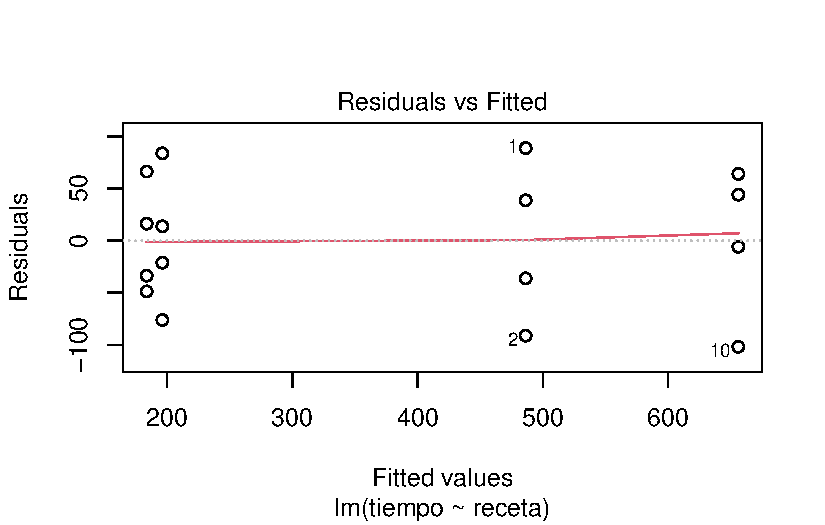
\includegraphics{solucion-masa-pizza_files/figure-pdf/graf-modelo-1-1.pdf}

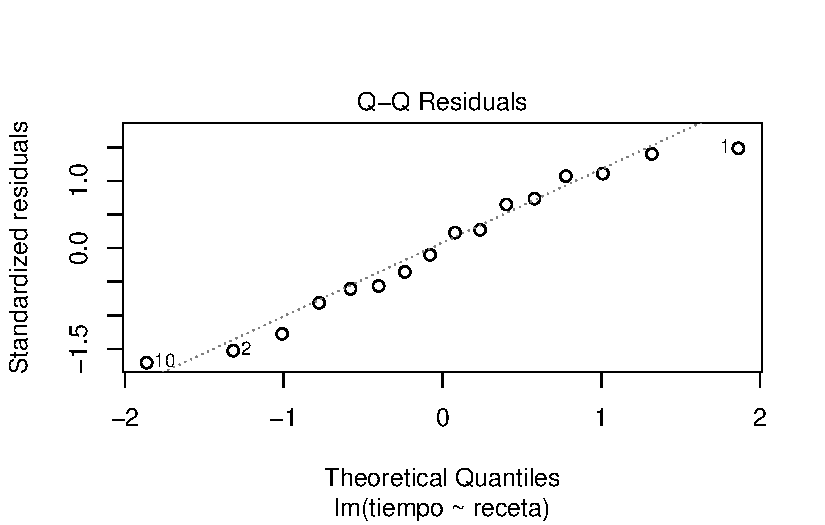
\includegraphics{solucion-masa-pizza_files/figure-pdf/graf-modelo-1-2.pdf}

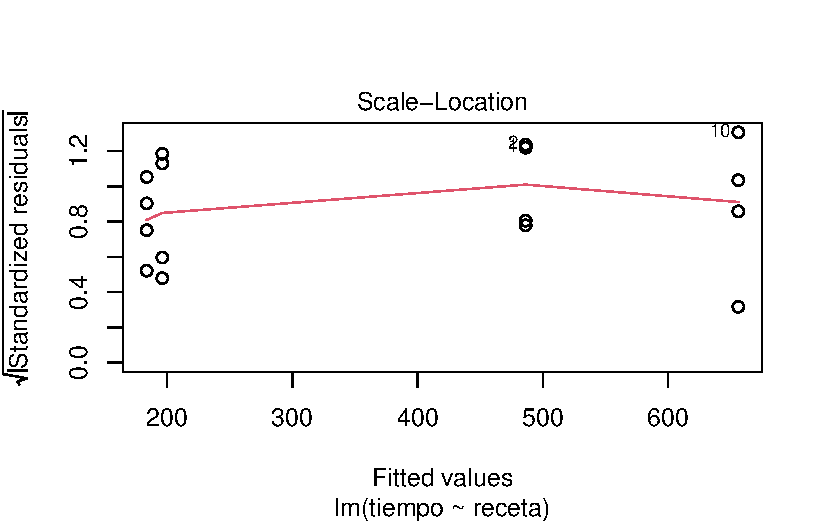
\includegraphics{solucion-masa-pizza_files/figure-pdf/graf-modelo-1-3.pdf}

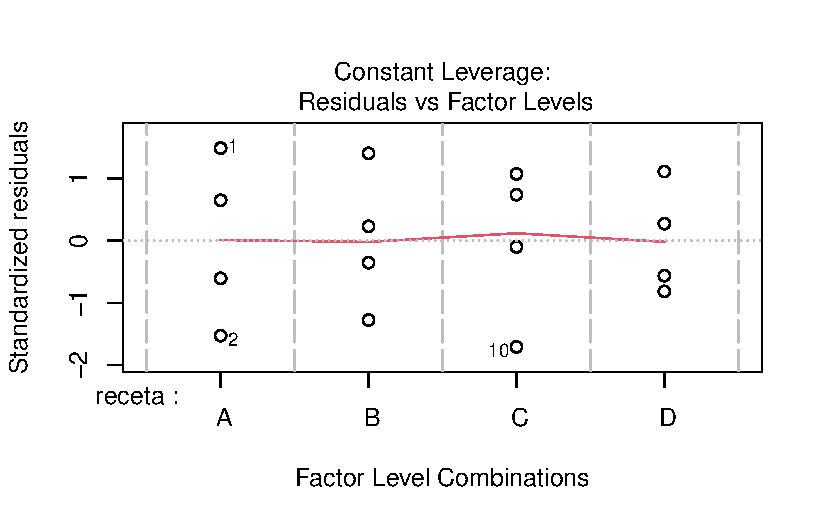
\includegraphics{solucion-masa-pizza_files/figure-pdf/graf-modelo-1-4.pdf}

Me parece que se ve un comportamiento bastante razonable en los
residuos. Si nos ponemos estrictos a lo mejor el supuesto de normalidad
en los residuos se ve un poco dudoso y quizás también un poco de
heterogeneidad de varianzas. Pero nada muy marcado como para invalidar
el ajuste del modelo.

Con los resultados anteriores puedo avanzar con bastante confianza para
atender la cuestión de \emph{cuál será la receta con la que la masa sube
más rápido}. La forma que elegí para hacer esto es seguir con un enfoque
de modelación, reformular el modelo original y valorar si cambia en
forma importante al redefinir el factor de recetas. Otras formas de
hacerlo serían el recurrir a pruebas t pareadas, que es lo que Fisher
llamó \emph{pruebas protegidas} por que ya rechazamos la omnibus
\textbf{H}0. Otra posibilidad es usar \texttt{TukeyHSD} de la biblioteca
\texttt{stats} (se carga al abrir \textbf{R} sin preguntarnos), o
podríamos recurrir a la
\href{https://towardsdatascience.com/anova-vs-bonferroni-correction-c8573936a64e}{corrección
de Boferroni}. Lo importante es no olvidar que cuando llegamos a este
punto, estas comparaciones las hacemos en un ámbito en gran parte
exploratorio. Por eso a mi me gusta mantenerme en el plan de que
\textbf{el modelo es la historia} y buscar producir un modelo que
incluya también esas comparaciones. Así lo hice. Por lo que vi en los
coeficientes estimados las recetas parecen diferir casi todas en
rendimiento, salvo la pareja \emph{B-D} que son las que dan tiempos más
cortos, por lo tanto, la pregunta que para mi sigue es si un modelo en
donde no distingo entre estas dos recetas, mantiene un buen ajuste a los
datos observados.

\begin{Shaded}
\begin{Highlighting}[]
\NormalTok{masa}\SpecialCharTok{$}\NormalTok{receta\_BD }\OtherTok{\textless{}{-}}\NormalTok{ masa}\SpecialCharTok{$}\NormalTok{receta}
\FunctionTok{levels}\NormalTok{(masa}\SpecialCharTok{$}\NormalTok{receta\_BD) }\OtherTok{\textless{}{-}} \FunctionTok{c}\NormalTok{(}\StringTok{"A"}\NormalTok{, }\StringTok{"BD"}\NormalTok{, }\StringTok{"C"}\NormalTok{, }\StringTok{"BD"}\NormalTok{)}

\NormalTok{masa\_lm\_BD }\OtherTok{\textless{}{-}} \FunctionTok{lm}\NormalTok{(tiempo }\SpecialCharTok{\textasciitilde{}}\NormalTok{ receta\_BD, }\AttributeTok{data =}\NormalTok{ masa)}
\FunctionTok{anova}\NormalTok{(masa\_lm\_BD, masa\_lm)}
\end{Highlighting}
\end{Shaded}

\begin{verbatim}
Analysis of Variance Table

Model 1: tiempo ~ receta_BD
Model 2: tiempo ~ receta
  Res.Df   RSS Df Sum of Sq      F Pr(>F)
1     13 57441                           
2     12 57128  1     312.5 0.0656 0.8021
\end{verbatim}

\begin{Shaded}
\begin{Highlighting}[]
\FunctionTok{summary}\NormalTok{(masa\_lm\_BD)}
\end{Highlighting}
\end{Shaded}

\begin{verbatim}

Call:
lm(formula = tiempo ~ receta_BD, data = masa)

Residuals:
    Min      1Q  Median      3Q     Max 
-102.00  -43.75    2.00   48.00   90.00 

Coefficients:
            Estimate Std. Error t value Pr(>|t|)    
(Intercept)   486.25      33.24  14.630 1.88e-09 ***
receta_BDBD  -296.25      40.71  -7.278 6.20e-06 ***
receta_BDC    169.75      47.00   3.611  0.00316 ** 
---
Signif. codes:  0 '***' 0.001 '**' 0.01 '*' 0.05 '.' 0.1 ' ' 1

Residual standard error: 66.47 on 13 degrees of freedom
Multiple R-squared:  0.9175,    Adjusted R-squared:  0.9048 
F-statistic: 72.27 on 2 and 13 DF,  p-value: 9.069e-08
\end{verbatim}

Este resultado me sugiere que hay una mínima pérdida de ajuste a los
datos y que el nuevo modelo podría considerarse prácticamente
equivalente a la versión más compleja que distingue cada receta. Así que
la proposición de que es razonable considerar a las recetas \emph{B} y
\emph{D} como equivalentes se puede defender. Al hacerlo no pierdo mucho
de correspondencia entre los valores que produce el nuevo modelo y los
datos. En realidad ya no me interesa averiguar que pasa con las otras
recetas, pues ambas tienen un desempeño más lento que las que he
indentificado, así que este modelo es el \textbf{mínimo adecuado para
esta historia}. ¿Se habrá producido alguna distorsión en otros aspectos
estadísticos del modelo?

\begin{Shaded}
\begin{Highlighting}[]
\FunctionTok{plot}\NormalTok{(masa\_lm\_BD)}
\end{Highlighting}
\end{Shaded}

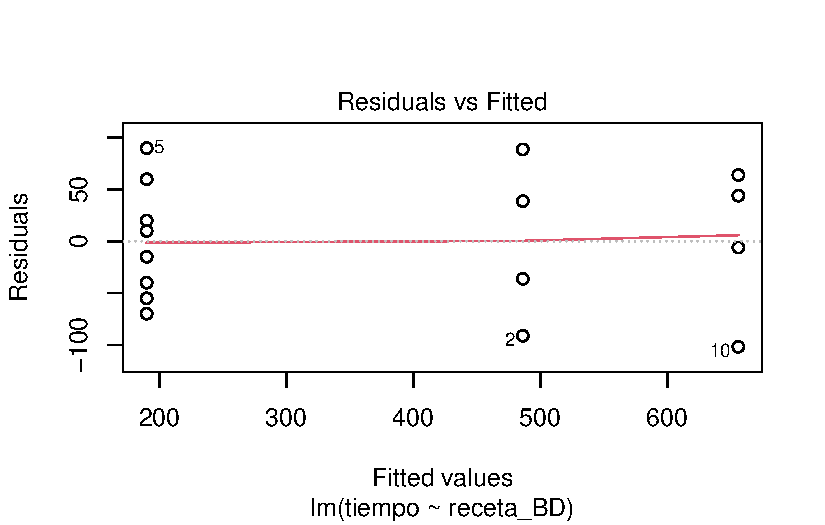
\includegraphics{solucion-masa-pizza_files/figure-pdf/graf-combo-recetas-1.pdf}

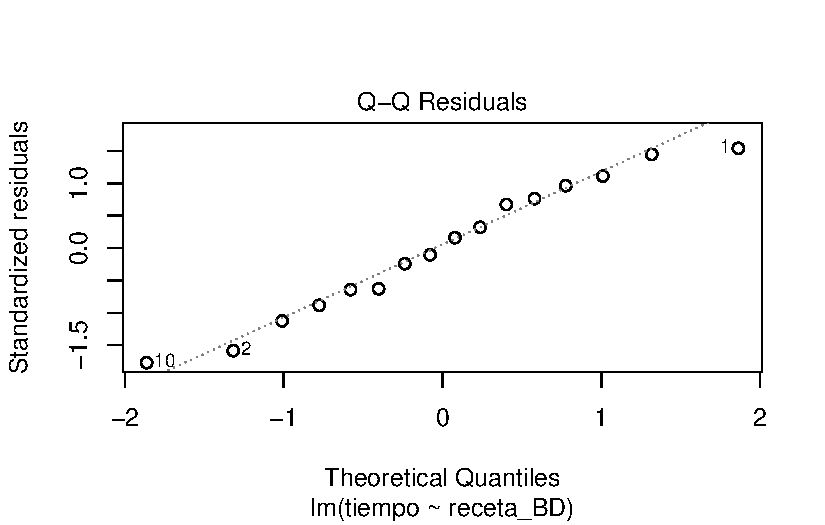
\includegraphics{solucion-masa-pizza_files/figure-pdf/graf-combo-recetas-2.pdf}

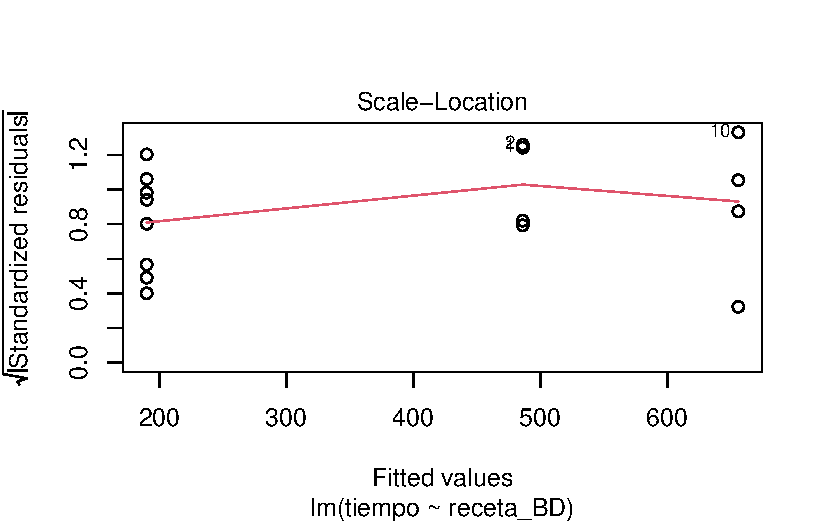
\includegraphics{solucion-masa-pizza_files/figure-pdf/graf-combo-recetas-3.pdf}

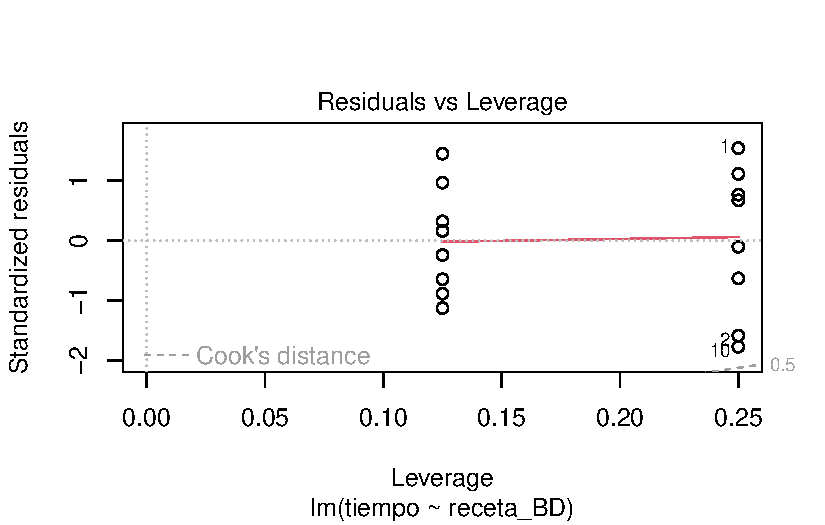
\includegraphics{solucion-masa-pizza_files/figure-pdf/graf-combo-recetas-4.pdf}

El comportamiento de los residuos se ve muy semejante al comportamiento
del modelo completo. Sigo sin ver mayores problemas en el ajuste. Es
cierto que se ven detallitos que hacen tener ligeras dudas, quizás
relacionados con heterocedasticidad. Así que hagamos algo al respecto,
aunque no sea más que con \textbf{fines didácticos}.

\subsection{Opciones avanzadas de
análisis}\label{opciones-avanzadas-de-anuxe1lisis}

\subsubsection{Modelo ponderado}\label{modelo-ponderado}

Lo que haremos es utilizar la opción \texttt{weight} de la función
\texttt{lm}, esto nos permite hacer lo que se llama \emph{modelos de
regresión ponderados}. Hay muchas posibles razones para utilizar
\emph{esquemas de ponderación}, todos relacionados con la idea de que
podemos proponer argumentos sobre qué datos deberían influir más sobre
el ajuste del modelo. En este caso utilizaremos la idea que anoté al
principio y que es relativamente común encontrarla en la práctica.
Muchas veces pasa que cuando el tamaño de la respuesta aumenta también
lo hace la variación con la que la observamos. Es decir a mayor media,
mayor varianza. En el modelo ponderado lo podemos expresar pensando que
deberíamos darle menos credibilidad (peso) a las observaciones asociadas
con tratamientos que producen medias más grandes.

A continuación les muestro como pondríamos estas ideas en práctica con
\texttt{lm}. Lo que haré es construir una expresión que relacione el
tamaño de los residuos con las medias de los tratamientos, lo que me
permitirá estimar algo parecido a las varianzas asociadas con cada
tratamiento en el modelo. A partir de ahí construyo la variable de
ponderación que será un expresión relacionada con:

\[
  ponderador \propto  \frac{1}{\sigma ^2}
\]

\begin{Shaded}
\begin{Highlighting}[]
\CommentTok{\# Modelo ponderado para enfrentarnos a la heterocedasticidad}
\CommentTok{\# Defino los ponderadores a usar}
\NormalTok{pond }\OtherTok{\textless{}{-}} \DecValTok{1} \SpecialCharTok{/} \FunctionTok{lm}\NormalTok{(}\FunctionTok{abs}\NormalTok{(masa\_lm}\SpecialCharTok{$}\NormalTok{residuals) }\SpecialCharTok{\textasciitilde{}}\NormalTok{ masa\_lm}\SpecialCharTok{$}\NormalTok{fitted.values)}\SpecialCharTok{$}\NormalTok{fitted.values}\SpecialCharTok{\^{}}\DecValTok{2}

\CommentTok{\# Ajusto un modelo ponderando dando mayor peso a los tratamientos con menor varianza}
\NormalTok{masa\_lm\_pond }\OtherTok{\textless{}{-}} \FunctionTok{lm}\NormalTok{(tiempo }\SpecialCharTok{\textasciitilde{}}\NormalTok{ receta, }\AttributeTok{data =}\NormalTok{ masa, }\AttributeTok{weights =}\NormalTok{ pond)}
\FunctionTok{anova}\NormalTok{(masa\_lm\_pond)}
\end{Highlighting}
\end{Shaded}

\begin{verbatim}
Analysis of Variance Table

Response: tiempo
          Df  Sum Sq Mean Sq F value    Pr(>F)    
receta     3 223.626  74.542  42.822 1.097e-06 ***
Residuals 12  20.889   1.741                      
---
Signif. codes:  0 '***' 0.001 '**' 0.01 '*' 0.05 '.' 0.1 ' ' 1
\end{verbatim}

\begin{Shaded}
\begin{Highlighting}[]
\FunctionTok{summary}\NormalTok{(masa\_lm\_pond)}
\end{Highlighting}
\end{Shaded}

\begin{verbatim}

Call:
lm(formula = tiempo ~ receta, data = masa, weights = pond)

Weighted Residuals:
     Min       1Q   Median       3Q      Max 
-1.70827 -0.80847  0.09686  0.82064  1.79195 

Coefficients:
            Estimate Std. Error t value Pr(>|t|)    
(Intercept)   486.25      36.23  13.421 1.38e-08 ***
receta B     -290.00      47.57  -6.096 5.37e-05 ***
receta C      169.75      53.52   3.172  0.00804 ** 
receta D     -302.50      47.42  -6.379 3.51e-05 ***
---
Signif. codes:  0 '***' 0.001 '**' 0.01 '*' 0.05 '.' 0.1 ' ' 1

Residual standard error: 1.319 on 12 degrees of freedom
Multiple R-squared:  0.9146,    Adjusted R-squared:  0.8932 
F-statistic: 42.82 on 3 and 12 DF,  p-value: 1.097e-06
\end{verbatim}

\begin{Shaded}
\begin{Highlighting}[]
\FunctionTok{plot}\NormalTok{((masa\_lm\_pond))}
\end{Highlighting}
\end{Shaded}

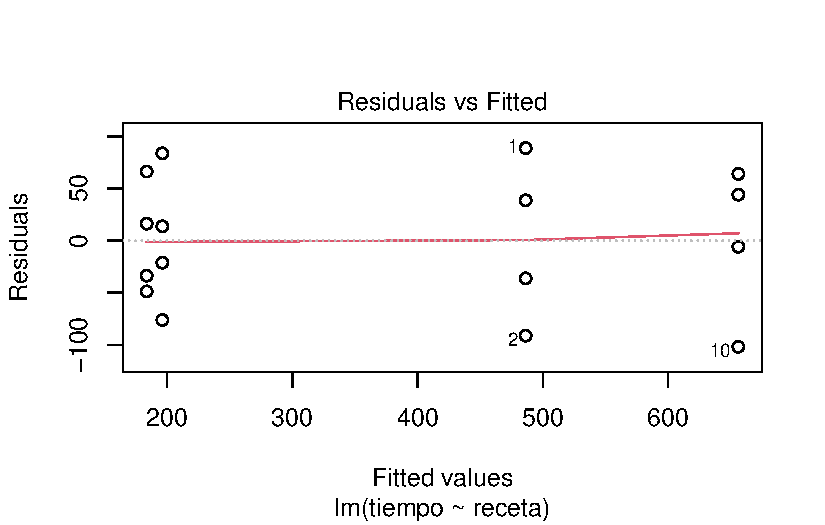
\includegraphics{solucion-masa-pizza_files/figure-pdf/modelo-pond-1.pdf}

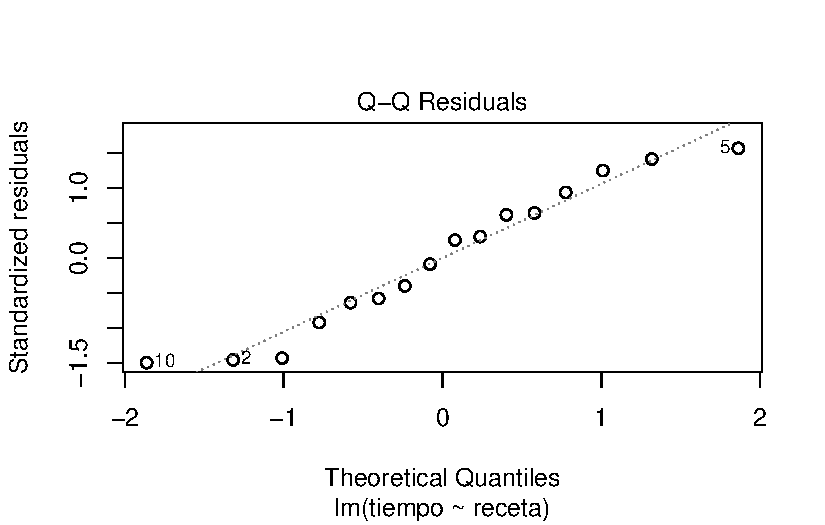
\includegraphics{solucion-masa-pizza_files/figure-pdf/modelo-pond-2.pdf}

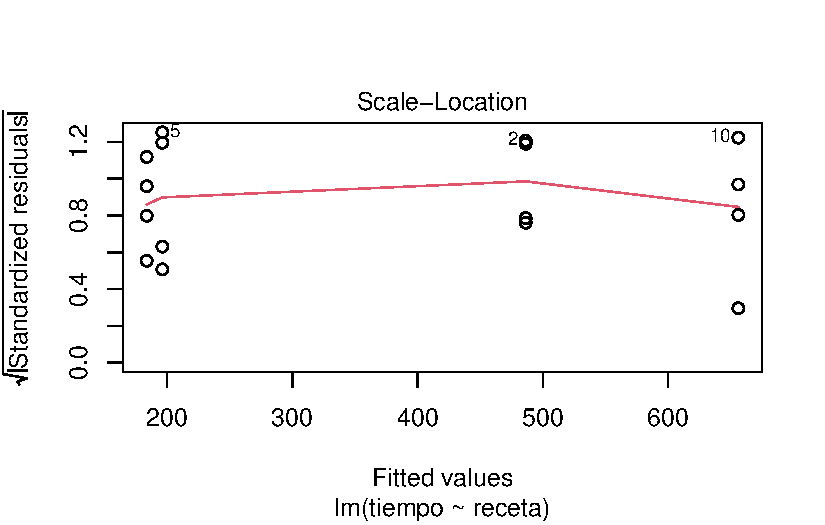
\includegraphics{solucion-masa-pizza_files/figure-pdf/modelo-pond-3.pdf}

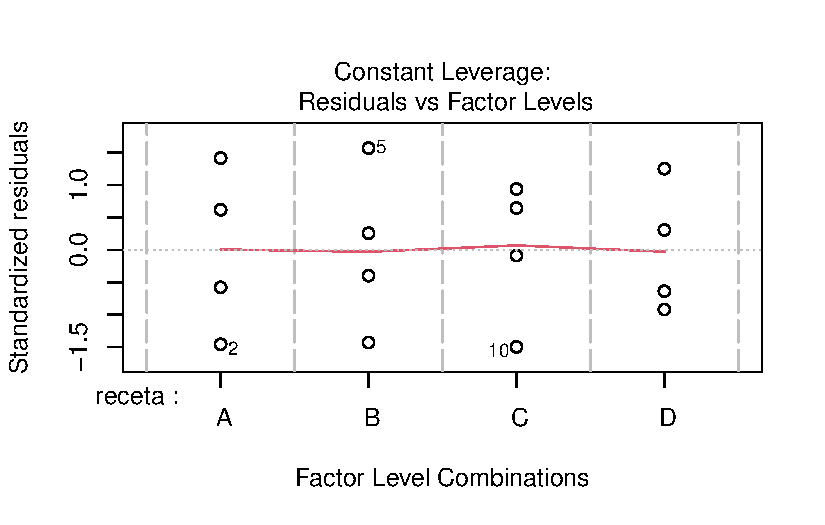
\includegraphics{solucion-masa-pizza_files/figure-pdf/modelo-pond-4.pdf}

Como cabría esperar, este modelo pierde un poco en ajuste, pero nada
preocupante. Los resultados sostienen la misma historia que habíamos
encontrado en el enfoque no ponderado y en todo caso se aprecia una
pequeña mejora en cuanto a la preocupación de que hubiera
heterocedasticidad en los datos y esto pudiera estar afectando los
resultados.

Para completar el análisis hago la valoración de la relevancia de
separar las recetas \emph{B} y \emph{D} del resto. Considerando los
mismos ponderadores que use con el modelo completo.

\begin{Shaded}
\begin{Highlighting}[]
\CommentTok{\# Ajusto un modelo ponderado con mayor peso los tratamientos con menor varianza}
\NormalTok{masa\_lm\_BD\_pond }\OtherTok{\textless{}{-}} \FunctionTok{lm}\NormalTok{(tiempo }\SpecialCharTok{\textasciitilde{}}\NormalTok{ receta\_BD, }\AttributeTok{data =}\NormalTok{ masa, }\AttributeTok{weights =}\NormalTok{ pond)}
\FunctionTok{anova}\NormalTok{(masa\_lm\_pond, masa\_lm\_BD\_pond)}
\end{Highlighting}
\end{Shaded}

\begin{verbatim}
Analysis of Variance Table

Model 1: tiempo ~ receta
Model 2: tiempo ~ receta_BD
  Res.Df    RSS Df Sum of Sq      F Pr(>F)
1     12 20.889                           
2     13 21.033 -1  -0.14415 0.0828 0.7784
\end{verbatim}

\begin{Shaded}
\begin{Highlighting}[]
\FunctionTok{summary}\NormalTok{(masa\_lm\_BD\_pond)}
\end{Highlighting}
\end{Shaded}

\begin{verbatim}

Call:
lm(formula = tiempo ~ receta_BD, data = masa, weights = pond)

Weighted Residuals:
     Min       1Q   Median       3Q      Max 
-1.70827 -0.94219  0.05806  0.82064  1.92669 

Coefficients:
            Estimate Std. Error t value Pr(>|t|)    
(Intercept)   486.25      34.93  13.921 3.45e-09 ***
receta_BDBD  -296.30      40.72  -7.276 6.22e-06 ***
receta_BDC    169.75      51.59   3.290  0.00586 ** 
---
Signif. codes:  0 '***' 0.001 '**' 0.01 '*' 0.05 '.' 0.1 ' ' 1

Residual standard error: 1.272 on 13 degrees of freedom
Multiple R-squared:  0.914, Adjusted R-squared:  0.9007 
F-statistic: 69.06 on 2 and 13 DF,  p-value: 1.188e-07
\end{verbatim}

\begin{Shaded}
\begin{Highlighting}[]
\FunctionTok{plot}\NormalTok{((masa\_lm\_BD\_pond))}
\end{Highlighting}
\end{Shaded}

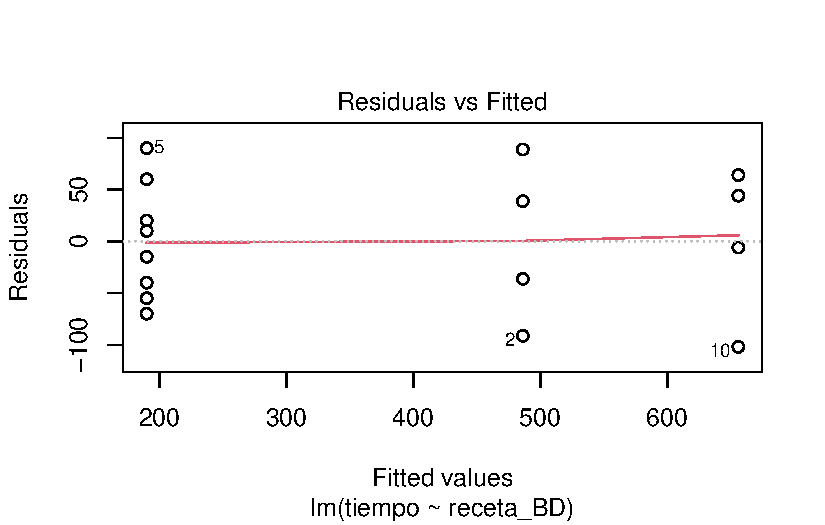
\includegraphics{solucion-masa-pizza_files/figure-pdf/modPond-combo-1.pdf}

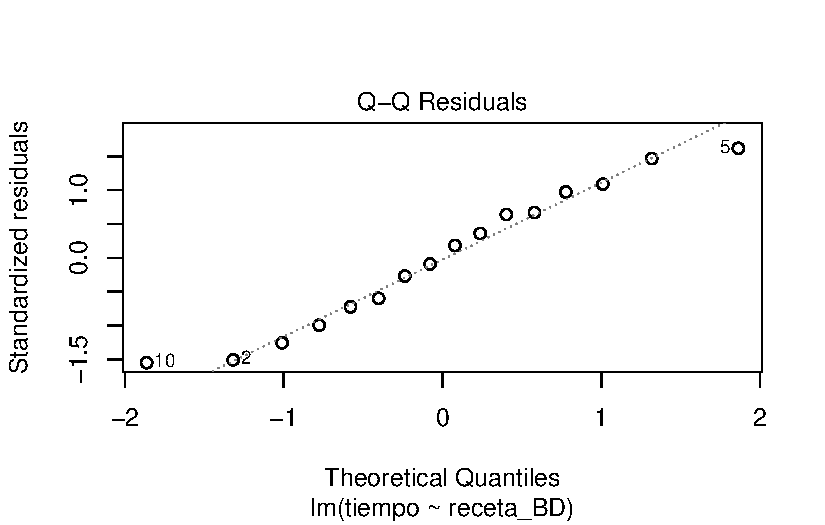
\includegraphics{solucion-masa-pizza_files/figure-pdf/modPond-combo-2.pdf}

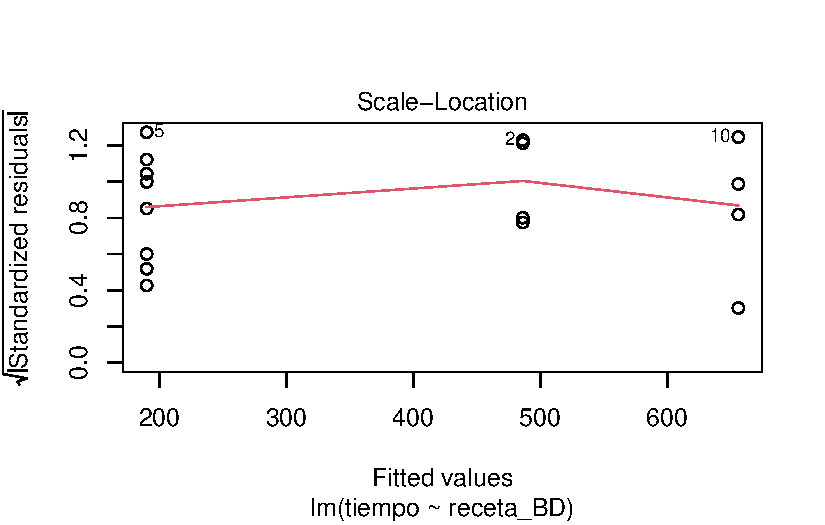
\includegraphics{solucion-masa-pizza_files/figure-pdf/modPond-combo-3.pdf}

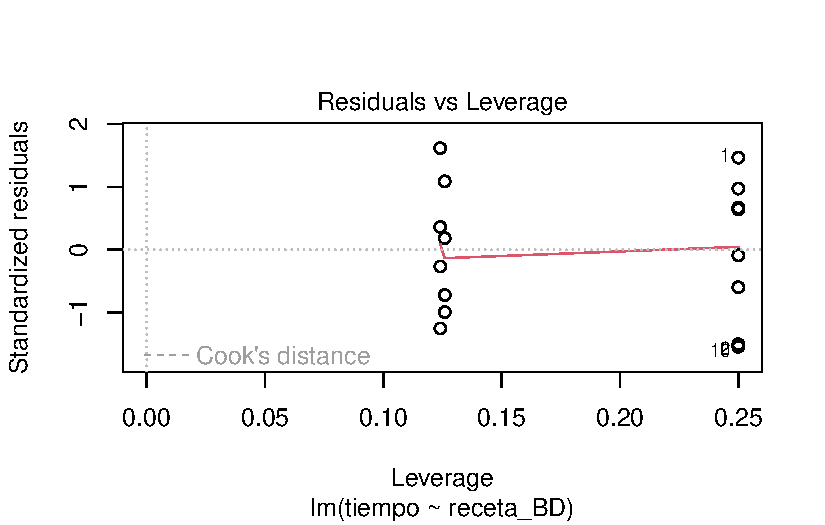
\includegraphics{solucion-masa-pizza_files/figure-pdf/modPond-combo-4.pdf}

Los resultados se sostienen. Quizás ahora la falta de normalidad podría
ser una inquietud, pero dada la congruencia entre los resultados de los
varios modelos, sospecho que no está afectando fundamentalmente la
naturaleza del patrón que estamos detectando. Marcelo debería tener
mucha confianza al afirmar que las recetas \emph{B} y \emph{D} tiene un
mejor desempeño que las otras dos y que entre estas dos no hay una
diferencia detectable.

\subsubsection{Offset: Modelo
``redondeado''}\label{offset-modelo-redondeado}

Un último asunto ¿cómo puedo poner a prueba hipótesis de interés que no
sean la \emph{H}0=0?. Una manera es recurrir a la opción \texttt{offset}
en \textbf{R}. A continuación muestro una forma de hacerlo. Lo que haré
es tomar los coeficientes estimados y redondearlos, para ver que tanto
de la capacidad predictiva del ajuste se pierde en la \emph{versión
simplificada} por el acto de redondear o incluso optando por usar
coeficientes \emph{fáciles de recordar}.

\begin{Shaded}
\begin{Highlighting}[]
\CommentTok{\# Tomo los coeficientes estimados del modelo y elimino todos los decimales}
\NormalTok{coef\_BD\_pond }\OtherTok{\textless{}{-}} \FunctionTok{round}\NormalTok{(}\FunctionTok{coef}\NormalTok{(masa\_lm\_BD\_pond), }\DecValTok{0}\NormalTok{)}
\FunctionTok{names}\NormalTok{(coef\_BD\_pond) }\OtherTok{\textless{}{-}}  \FunctionTok{names}\NormalTok{(}\FunctionTok{coef}\NormalTok{(masa\_lm\_BD\_pond))}

\NormalTok{coef\_BD\_pond\_facil }\OtherTok{\textless{}{-}} \FunctionTok{c}\NormalTok{(}\DecValTok{490}\NormalTok{, }\SpecialCharTok{{-}}\DecValTok{300}\NormalTok{, }\DecValTok{170}\NormalTok{)}
\FunctionTok{names}\NormalTok{(coef\_BD\_pond\_facil) }\OtherTok{\textless{}{-}} \FunctionTok{names}\NormalTok{(}\FunctionTok{coef}\NormalTok{(masa\_lm\_BD\_pond))}
\end{Highlighting}
\end{Shaded}

Como vimos en clase, puedo obtener la matriz de variables explicativas
(\emph{dummy} o no) incluidas en el modelo con la función
\texttt{model.matrix}. Si multiplico las columnas de esta matriz por el
coeficiente que le corresponde (multiplicación normal, no matricial),
tengo una nueva matriz que contiene en cada renglón, el valor que
predice el modelo ajustado para la observación correspondiente.

\begin{Shaded}
\begin{Highlighting}[]
\CommentTok{\# La matriz del modelo es esta}
\NormalTok{bd\_pond\_mat }\OtherTok{\textless{}{-}} \FunctionTok{model.matrix}\NormalTok{(masa\_lm\_BD\_pond)}


\CommentTok{\# Ahora tenemos que armar la matriz con el modelo para cada renglón}
\NormalTok{mode\_off }\OtherTok{\textless{}{-}}  \FunctionTok{data.frame}\NormalTok{(}\AttributeTok{intercept =}\NormalTok{ coef\_BD\_pond[}\DecValTok{1}\NormalTok{] }\SpecialCharTok{*}\NormalTok{ bd\_pond\_mat[, }\DecValTok{1}\NormalTok{],}
                        \AttributeTok{receta\_BD =}\NormalTok{ coef\_BD\_pond[}\DecValTok{2}\NormalTok{] }\SpecialCharTok{*}\NormalTok{ bd\_pond\_mat[, }\DecValTok{2}\NormalTok{],}
                        \AttributeTok{receta\_C  =}\NormalTok{ coef\_BD\_pond[}\DecValTok{3}\NormalTok{] }\SpecialCharTok{*}\NormalTok{ bd\_pond\_mat[, }\DecValTok{3}\NormalTok{])}
\NormalTok{mode\_off}
\end{Highlighting}
\end{Shaded}

\begin{verbatim}
   intercept receta_BD receta_C
1        486         0        0
2        486         0        0
3        486         0        0
4        486         0        0
5        486      -296        0
6        486      -296        0
7        486      -296        0
8        486      -296        0
9        486         0      170
10       486         0      170
11       486         0      170
12       486         0      170
13       486      -296        0
14       486      -296        0
15       486      -296        0
16       486      -296        0
\end{verbatim}

\begin{Shaded}
\begin{Highlighting}[]
\CommentTok{\# Otra forma de hacer esto mismo es esta}
\NormalTok{mode\_off\_2 }\OtherTok{\textless{}{-}} \FunctionTok{t}\NormalTok{(coef\_BD\_pond }\SpecialCharTok{*} \FunctionTok{t}\NormalTok{(}\FunctionTok{model.matrix}\NormalTok{(masa\_lm\_BD\_pond)))}

\NormalTok{mode\_off\_2 }\SpecialCharTok{==}\NormalTok{ mode\_off}
\end{Highlighting}
\end{Shaded}

\begin{verbatim}
   intercept receta_BD receta_C
1       TRUE      TRUE     TRUE
2       TRUE      TRUE     TRUE
3       TRUE      TRUE     TRUE
4       TRUE      TRUE     TRUE
5       TRUE      TRUE     TRUE
6       TRUE      TRUE     TRUE
7       TRUE      TRUE     TRUE
8       TRUE      TRUE     TRUE
9       TRUE      TRUE     TRUE
10      TRUE      TRUE     TRUE
11      TRUE      TRUE     TRUE
12      TRUE      TRUE     TRUE
13      TRUE      TRUE     TRUE
14      TRUE      TRUE     TRUE
15      TRUE      TRUE     TRUE
16      TRUE      TRUE     TRUE
\end{verbatim}

\begin{Shaded}
\begin{Highlighting}[]
\CommentTok{\# modelo con offcets fáciles de recordar}
\NormalTok{mode\_off\_facil }\OtherTok{\textless{}{-}} \FunctionTok{t}\NormalTok{(coef\_BD\_pond\_facil }\SpecialCharTok{*} \FunctionTok{t}\NormalTok{(}\FunctionTok{model.matrix}\NormalTok{(masa\_lm\_BD\_pond)))}
\end{Highlighting}
\end{Shaded}

Ahora pongamos a prueba que tan bien funciona esta versión
\emph{redondeada} del modelo que hemos ajustado.

\begin{Shaded}
\begin{Highlighting}[]
\CommentTok{\# valora{-}modelos}

\FunctionTok{library}\NormalTok{(flextable, }\AttributeTok{warn.conflicts =} \ConstantTok{FALSE}\NormalTok{)}

\NormalTok{masa\_lm\_BD\_pond\_off }\OtherTok{\textless{}{-}} \FunctionTok{lm}\NormalTok{(tiempo }\SpecialCharTok{\textasciitilde{}} \SpecialCharTok{{-}}\DecValTok{1}\NormalTok{, }\AttributeTok{data =}\NormalTok{ masa, }
                        \AttributeTok{weights =}\NormalTok{ pond, }
                        \AttributeTok{offset =}\NormalTok{ (mode\_off[,}\DecValTok{1}\NormalTok{] }\SpecialCharTok{+}\NormalTok{ mode\_off[,}\DecValTok{2}\NormalTok{] }\SpecialCharTok{+} 
\NormalTok{                                  mode\_off[, }\DecValTok{3}\NormalTok{]))}

\NormalTok{masa\_lm\_BD\_pond\_off\_facil }\OtherTok{\textless{}{-}} \FunctionTok{lm}\NormalTok{(tiempo }\SpecialCharTok{\textasciitilde{}} \SpecialCharTok{{-}}\DecValTok{1}\NormalTok{, }\AttributeTok{data =}\NormalTok{ masa, }
                        \AttributeTok{weights =}\NormalTok{ pond, }
                        \AttributeTok{offset =}\NormalTok{ (mode\_off\_facil[,}\DecValTok{1}\NormalTok{] }\SpecialCharTok{+}\NormalTok{ mode\_off\_facil[,}\DecValTok{2}\NormalTok{] }\SpecialCharTok{+} 
\NormalTok{                                  mode\_off\_facil[, }\DecValTok{3}\NormalTok{]))}

\NormalTok{resumen }\OtherTok{\textless{}{-}} \FunctionTok{as\_tibble\_row}\NormalTok{(}\FunctionTok{coef}\NormalTok{(masa\_lm\_BD\_pond)) }\SpecialCharTok{\%\textgreater{}\%}
           \FunctionTok{bind\_rows}\NormalTok{(coef\_BD\_pond, }
\NormalTok{                     coef\_BD\_pond\_facil) }\SpecialCharTok{\%\textgreater{}\%} 
           \FunctionTok{bind\_cols}\NormalTok{(}\StringTok{\textasciigrave{}}\AttributeTok{Pr(\textgreater{}F)}\StringTok{\textasciigrave{}} \OtherTok{=} \FunctionTok{c}\NormalTok{(}\DecValTok{0}\NormalTok{, }
                       \FunctionTok{anova}\NormalTok{(masa\_lm\_BD\_pond, masa\_lm\_BD\_pond\_off)}\SpecialCharTok{$}\StringTok{\textasciigrave{}}\AttributeTok{Pr(\textgreater{}F)}\StringTok{\textasciigrave{}}\NormalTok{[}\DecValTok{2}\NormalTok{],}
                       \FunctionTok{anova}\NormalTok{(masa\_lm\_BD\_pond, masa\_lm\_BD\_pond\_off\_facil)}\SpecialCharTok{$}\StringTok{\textasciigrave{}}\AttributeTok{Pr(\textgreater{}F)}\StringTok{\textasciigrave{}}\NormalTok{[}\DecValTok{2}\NormalTok{]),}
                     \AttributeTok{modelo =} \FunctionTok{c}\NormalTok{(}\StringTok{"Ajuste"}\NormalTok{, }\StringTok{"Redondeo"}\NormalTok{, }\StringTok{"Fácil"}\NormalTok{)) }\SpecialCharTok{\%\textgreater{}\%} 
           \FunctionTok{select}\NormalTok{(}\FunctionTok{c}\NormalTok{(}\DecValTok{5}\NormalTok{,}\DecValTok{1}\SpecialCharTok{:}\DecValTok{3}\NormalTok{,}\DecValTok{4}\NormalTok{)) }\SpecialCharTok{\%\textgreater{}\%} 
           \FunctionTok{flextable}\NormalTok{() }\SpecialCharTok{\%\textgreater{}\%} 
           \FunctionTok{set\_header\_labels}\NormalTok{(}\StringTok{"(Intercept)"} \OtherTok{=} \StringTok{"A (ref.)"}\NormalTok{, }
                             \AttributeTok{receta\_BDBD =} \StringTok{"BD"}\NormalTok{, }
                             \AttributeTok{receta\_BDC =} \StringTok{"C"}\NormalTok{) }\SpecialCharTok{\%\textgreater{}\%} 
           \FunctionTok{add\_header\_row}\NormalTok{(}\AttributeTok{colwidths =} \FunctionTok{c}\NormalTok{(}\DecValTok{1}\NormalTok{, }\DecValTok{3}\NormalTok{, }\DecValTok{1}\NormalTok{),}
                          \AttributeTok{values =} \FunctionTok{c}\NormalTok{(}\StringTok{""}\NormalTok{, }\StringTok{"Receta (tiempo)"}\NormalTok{, }\StringTok{"Pr"}\NormalTok{),}
                          \AttributeTok{top =} \ConstantTok{TRUE}\NormalTok{) }\SpecialCharTok{\%\textgreater{}\%}
           \FunctionTok{theme\_zebra}\NormalTok{() }\SpecialCharTok{\%\textgreater{}\%} 
           \FunctionTok{vline}\NormalTok{(}\AttributeTok{j =} \FunctionTok{c}\NormalTok{(}\DecValTok{1}\NormalTok{,}\DecValTok{4}\NormalTok{)) }


\NormalTok{resumen}
\end{Highlighting}
\end{Shaded}

\global\setlength{\Oldarrayrulewidth}{\arrayrulewidth}

\global\setlength{\Oldtabcolsep}{\tabcolsep}

\setlength{\tabcolsep}{2pt}

\renewcommand*{\arraystretch}{1.5}



\providecommand{\ascline}[3]{\noalign{\global\arrayrulewidth #1}\arrayrulecolor[HTML]{#2}\cline{#3}}

\begin{longtable}[c]{|p{0.75in}|p{0.75in}|p{0.75in}|p{0.75in}|p{0.75in}}

\caption{\label{tbl-eval-modelo}Comparación del desempeño de
estimadores}

\tabularnewline

\hhline{>{\arrayrulecolor[HTML]{000000}\global\arrayrulewidth=0pt}->{\arrayrulecolor[HTML]{000000}\global\arrayrulewidth=0pt}->{\arrayrulecolor[HTML]{000000}\global\arrayrulewidth=0pt}->{\arrayrulecolor[HTML]{000000}\global\arrayrulewidth=0pt}->{\arrayrulecolor[HTML]{000000}\global\arrayrulewidth=0pt}-}

\multicolumn{1}{>{\cellcolor[HTML]{CFCFCF}\raggedright}m{\dimexpr 0.75in+0\tabcolsep}}{\textcolor[HTML]{000000}{\fontsize{11}{11}\selectfont{\global\setmainfont{Arial}{\textbf{}}}}} & \multicolumn{3}{!{\color[HTML]{666666}\vrule width 1pt}>{\cellcolor[HTML]{CFCFCF}\raggedleft}m{\dimexpr 2.25in+4\tabcolsep}}{\textcolor[HTML]{000000}{\fontsize{11}{11}\selectfont{\global\setmainfont{Arial}{\textbf{Receta\ (tiempo)}}}}} & \multicolumn{1}{!{\color[HTML]{666666}\vrule width 1pt}>{\cellcolor[HTML]{CFCFCF}\raggedleft}m{\dimexpr 0.75in+0\tabcolsep}}{\textcolor[HTML]{000000}{\fontsize{11}{11}\selectfont{\global\setmainfont{Arial}{\textbf{Pr}}}}} \\

\noalign{\global\arrayrulewidth 0pt}\arrayrulecolor[HTML]{000000}





\multicolumn{1}{>{\raggedright}m{\dimexpr 0.75in+0\tabcolsep}}{\textcolor[HTML]{000000}{\fontsize{11}{11}\selectfont{\global\setmainfont{Arial}{\textbf{modelo}}}}} & \multicolumn{1}{!{\color[HTML]{666666}\vrule width 1pt}>{\raggedleft}m{\dimexpr 0.75in+0\tabcolsep}}{\textcolor[HTML]{000000}{\fontsize{11}{11}\selectfont{\global\setmainfont{Arial}{\textbf{A\ (ref.)}}}}} & \multicolumn{1}{>{\raggedleft}m{\dimexpr 0.75in+0\tabcolsep}}{\textcolor[HTML]{000000}{\fontsize{11}{11}\selectfont{\global\setmainfont{Arial}{\textbf{BD}}}}} & \multicolumn{1}{>{\raggedleft}m{\dimexpr 0.75in+0\tabcolsep}}{\textcolor[HTML]{000000}{\fontsize{11}{11}\selectfont{\global\setmainfont{Arial}{\textbf{C}}}}} & \multicolumn{1}{!{\color[HTML]{666666}\vrule width 1pt}>{\raggedleft}m{\dimexpr 0.75in+0\tabcolsep}}{\textcolor[HTML]{000000}{\fontsize{11}{11}\selectfont{\global\setmainfont{Arial}{\textbf{Pr(>F)}}}}} \\

\noalign{\global\arrayrulewidth 0pt}\arrayrulecolor[HTML]{000000}

\endfirsthead 

\hhline{>{\arrayrulecolor[HTML]{000000}\global\arrayrulewidth=0pt}->{\arrayrulecolor[HTML]{000000}\global\arrayrulewidth=0pt}->{\arrayrulecolor[HTML]{000000}\global\arrayrulewidth=0pt}->{\arrayrulecolor[HTML]{000000}\global\arrayrulewidth=0pt}->{\arrayrulecolor[HTML]{000000}\global\arrayrulewidth=0pt}-}

\multicolumn{1}{>{\cellcolor[HTML]{CFCFCF}\raggedright}m{\dimexpr 0.75in+0\tabcolsep}}{\textcolor[HTML]{000000}{\fontsize{11}{11}\selectfont{\global\setmainfont{Arial}{\textbf{}}}}} & \multicolumn{3}{!{\color[HTML]{666666}\vrule width 1pt}>{\cellcolor[HTML]{CFCFCF}\raggedleft}m{\dimexpr 2.25in+4\tabcolsep}}{\textcolor[HTML]{000000}{\fontsize{11}{11}\selectfont{\global\setmainfont{Arial}{\textbf{Receta\ (tiempo)}}}}} & \multicolumn{1}{!{\color[HTML]{666666}\vrule width 1pt}>{\cellcolor[HTML]{CFCFCF}\raggedleft}m{\dimexpr 0.75in+0\tabcolsep}}{\textcolor[HTML]{000000}{\fontsize{11}{11}\selectfont{\global\setmainfont{Arial}{\textbf{Pr}}}}} \\

\noalign{\global\arrayrulewidth 0pt}\arrayrulecolor[HTML]{000000}





\multicolumn{1}{>{\raggedright}m{\dimexpr 0.75in+0\tabcolsep}}{\textcolor[HTML]{000000}{\fontsize{11}{11}\selectfont{\global\setmainfont{Arial}{\textbf{modelo}}}}} & \multicolumn{1}{!{\color[HTML]{666666}\vrule width 1pt}>{\raggedleft}m{\dimexpr 0.75in+0\tabcolsep}}{\textcolor[HTML]{000000}{\fontsize{11}{11}\selectfont{\global\setmainfont{Arial}{\textbf{A\ (ref.)}}}}} & \multicolumn{1}{>{\raggedleft}m{\dimexpr 0.75in+0\tabcolsep}}{\textcolor[HTML]{000000}{\fontsize{11}{11}\selectfont{\global\setmainfont{Arial}{\textbf{BD}}}}} & \multicolumn{1}{>{\raggedleft}m{\dimexpr 0.75in+0\tabcolsep}}{\textcolor[HTML]{000000}{\fontsize{11}{11}\selectfont{\global\setmainfont{Arial}{\textbf{C}}}}} & \multicolumn{1}{!{\color[HTML]{666666}\vrule width 1pt}>{\raggedleft}m{\dimexpr 0.75in+0\tabcolsep}}{\textcolor[HTML]{000000}{\fontsize{11}{11}\selectfont{\global\setmainfont{Arial}{\textbf{Pr(>F)}}}}} \\

\noalign{\global\arrayrulewidth 0pt}\arrayrulecolor[HTML]{000000}

\endhead



\multicolumn{1}{>{\cellcolor[HTML]{EFEFEF}\raggedright}m{\dimexpr 0.75in+0\tabcolsep}}{\textcolor[HTML]{000000}{\fontsize{11}{11}\selectfont{\global\setmainfont{Arial}{Ajuste}}}} & \multicolumn{1}{!{\color[HTML]{666666}\vrule width 1pt}>{\cellcolor[HTML]{EFEFEF}\raggedleft}m{\dimexpr 0.75in+0\tabcolsep}}{\textcolor[HTML]{000000}{\fontsize{11}{11}\selectfont{\global\setmainfont{Arial}{486.25}}}} & \multicolumn{1}{>{\cellcolor[HTML]{EFEFEF}\raggedleft}m{\dimexpr 0.75in+0\tabcolsep}}{\textcolor[HTML]{000000}{\fontsize{11}{11}\selectfont{\global\setmainfont{Arial}{-296.2973}}}} & \multicolumn{1}{>{\cellcolor[HTML]{EFEFEF}\raggedleft}m{\dimexpr 0.75in+0\tabcolsep}}{\textcolor[HTML]{000000}{\fontsize{11}{11}\selectfont{\global\setmainfont{Arial}{169.75}}}} & \multicolumn{1}{!{\color[HTML]{666666}\vrule width 1pt}>{\cellcolor[HTML]{EFEFEF}\raggedleft}m{\dimexpr 0.75in+0\tabcolsep}}{\textcolor[HTML]{000000}{\fontsize{11}{11}\selectfont{\global\setmainfont{Arial}{0.0000000}}}} \\

\noalign{\global\arrayrulewidth 0pt}\arrayrulecolor[HTML]{000000}





\multicolumn{1}{>{\raggedright}m{\dimexpr 0.75in+0\tabcolsep}}{\textcolor[HTML]{000000}{\fontsize{11}{11}\selectfont{\global\setmainfont{Arial}{Redondeo}}}} & \multicolumn{1}{!{\color[HTML]{666666}\vrule width 1pt}>{\raggedleft}m{\dimexpr 0.75in+0\tabcolsep}}{\textcolor[HTML]{000000}{\fontsize{11}{11}\selectfont{\global\setmainfont{Arial}{486.00}}}} & \multicolumn{1}{>{\raggedleft}m{\dimexpr 0.75in+0\tabcolsep}}{\textcolor[HTML]{000000}{\fontsize{11}{11}\selectfont{\global\setmainfont{Arial}{-296.0000}}}} & \multicolumn{1}{>{\raggedleft}m{\dimexpr 0.75in+0\tabcolsep}}{\textcolor[HTML]{000000}{\fontsize{11}{11}\selectfont{\global\setmainfont{Arial}{170.00}}}} & \multicolumn{1}{!{\color[HTML]{666666}\vrule width 1pt}>{\raggedleft}m{\dimexpr 0.75in+0\tabcolsep}}{\textcolor[HTML]{000000}{\fontsize{11}{11}\selectfont{\global\setmainfont{Arial}{0.9999999}}}} \\

\noalign{\global\arrayrulewidth 0pt}\arrayrulecolor[HTML]{000000}





\multicolumn{1}{>{\cellcolor[HTML]{EFEFEF}\raggedright}m{\dimexpr 0.75in+0\tabcolsep}}{\textcolor[HTML]{000000}{\fontsize{11}{11}\selectfont{\global\setmainfont{Arial}{Fácil}}}} & \multicolumn{1}{!{\color[HTML]{666666}\vrule width 1pt}>{\cellcolor[HTML]{EFEFEF}\raggedleft}m{\dimexpr 0.75in+0\tabcolsep}}{\textcolor[HTML]{000000}{\fontsize{11}{11}\selectfont{\global\setmainfont{Arial}{490.00}}}} & \multicolumn{1}{>{\cellcolor[HTML]{EFEFEF}\raggedleft}m{\dimexpr 0.75in+0\tabcolsep}}{\textcolor[HTML]{000000}{\fontsize{11}{11}\selectfont{\global\setmainfont{Arial}{-300.0000}}}} & \multicolumn{1}{>{\cellcolor[HTML]{EFEFEF}\raggedleft}m{\dimexpr 0.75in+0\tabcolsep}}{\textcolor[HTML]{000000}{\fontsize{11}{11}\selectfont{\global\setmainfont{Arial}{170.00}}}} & \multicolumn{1}{!{\color[HTML]{666666}\vrule width 1pt}>{\cellcolor[HTML]{EFEFEF}\raggedleft}m{\dimexpr 0.75in+0\tabcolsep}}{\textcolor[HTML]{000000}{\fontsize{11}{11}\selectfont{\global\setmainfont{Arial}{0.9990516}}}} \\

\noalign{\global\arrayrulewidth 0pt}\arrayrulecolor[HTML]{000000}




\end{longtable}

\arrayrulecolor[HTML]{000000}

\global\setlength{\arrayrulewidth}{\Oldarrayrulewidth}

\global\setlength{\tabcolsep}{\Oldtabcolsep}

\renewcommand*{\arraystretch}{1}

Como puedes ver funciona muy bien, es prácticamente indistinguible del
modelo ajustado con todas las cifras significativas que resultaron del
cálculo que hizo la computadora. Hay uun correspondencia término a
término entre el \emph{offset} y los coeficientes estimados y ahí
también puede verse que los coeficientes corresponden muy bien y dado el
\emph{offcet}, no habría razón para estimarlos con algún ajuste. Las
sumas de cuadrados residuales son prácticamente iguales en las dos
versiones del modelo, difiere muy poco, la probabilidad de que los
estimadores correspondan al mismo modelo es muy alta, mayor a 99.9\%. No
habría razón para no entregarle cualquiera de esa ecuaciones a Marcelo
para que hiciera cálculos futuros al preparar pizzas.

\subsection{Tarea}\label{tarea}

De hecho, ¿por qué no repetimos este experimento en casa? Se los
propongo como tarea y si les parece bien, habría que reunir los datos,
organizarlos para tenerlos en la nube de Google Drive y repetir
individualmente el proceso analítico que vimos aquí, por lo menos los
elementos básicos de la \emph{prueba de hipótesis}. A partir de la
experiencia, podremos empezar por discutir el diseño experimental,
convenir en lo que harán y podríamos finalmente discutir ideas sobre
\emph{reroducibilidad}, considerando los hallazgos de cada quién y de
todos en conjunto.

\begin{tcolorbox}[enhanced jigsaw, title=\textcolor{quarto-callout-tip-color}{\faLightbulb}\hspace{0.5em}{Pistas}, rightrule=.15mm, toptitle=1mm, toprule=.15mm, opacitybacktitle=0.6, bottomrule=.15mm, colbacktitle=quarto-callout-tip-color!10!white, colframe=quarto-callout-tip-color-frame, coltitle=black, opacityback=0, colback=white, breakable, bottomtitle=1mm, left=2mm, leftrule=.75mm, titlerule=0mm, arc=.35mm]

\begin{itemize}
\tightlist
\item
  Harina: 150 g
\item
  Agua: 50 ml
\item
  Leche: 25 ml
\item
  Azucar: 1/3 cdt
\item
  Levadura seca: 1/3 sobre (sobre de 11g)
\end{itemize}

\end{tcolorbox}



\end{document}
